\chapter{Energy Reconstruction}
\label{sec:energy}
	The~second stage of our reconstruction algorithm is the reconstruction of the~particle's energy using its reconstructed track (see section~\ref{sec:track}). We can achieve this by fitting the~track and extracting the~needed parameters of the~trajectory. We have tested three ways of reconstructing the~energy. Fitting is done using the~MINUIT algorithm implemented in ROOT~\cite{ROOT}. \textcolor{red}{Maybe cite some CERN article directly on MINUIT?}
	
	The~\textbf{Cubic Spline Fit} is a~rejected attempt at the~reconstruction of energy. It uses smoothly connected piecewise cubic polynomials between uniformly spaced nodes. Energy can then be computed using from the~fit parameters by computing the~radius of curvature in different points of the~fitted curve using the~known magnitude of the~magnetic field perpendicular to the trajectory. This approach was rejected because tuning the fit to have a~reasonably stable radius of curvature is unpractical.
	
	The~\textbf{Circle and Lines Fit} was chosen as an~alternative since this corresponds to the~shape of a~trajectory of a~charged particle moving through a~finite volume with a~homogeneous magnetic field. The~energy of the~particle can be estimated using the~fitted radius and the~magnitude of the~perpendicular magnetic field in the middle of the~\ac{TPC}.
	
	The~\textbf{Runge-Kutta Fit} uses the~4th order Runge-Kutta numerical integration described in section~\ref{sec:rks}. Initial parameters of the~track (including the~particle's energy) are optimized so that the~integrated trajectory fits to the~reconstructed one. This fit can also be performed as a~single parameter (energy) fit if we can get the initial position and orientation of the~particle on the~entrance to the~\ac{TPC} from previous detectors (\ac{Tpx3} and \ac{MWPC}, see section~\ref{sec:IEAP}).
	
	\begin{figure}
		\centering
		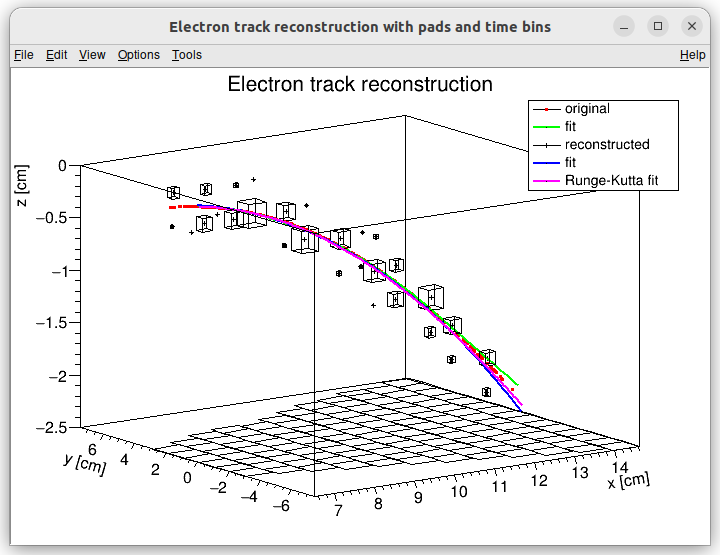
\includegraphics[width=0.5\textwidth]{9010_3d.png}
		\caption{Example of a~fitted reconstructed track. \textcolor{red}{Swap for better image.}}
		\label{fig:90103d}
	\end{figure}
	
	\section{Cubic Spline Fit}
		The~first attempt to get an~early estimate of the~kinetic energy of the~particle uses a~cubic spline fit. This approach was later rejected in favor of the~circle and lines fit described in section~\ref{sec:clines}. We use an~electron track starting in the origin of our coordinate system with an~initial direction in the~positive $x$~axis. The track is simulated microscopically (see section~\ref{sec:microsim}) with a~kinetic energy of 8~MeV in a~gas mixture 90\%~Ar~+~10\%~CO$_2$ (the~same track was used in section~\ref{sec:trackfirst}).
				
		In order to calculate the~spline, we use the~class \textit{TSpline3} from ROOT. This allows us to evaluate the~spline using the~coordinates $(x_n,z_n)$ of each node and the derivatives $d_1,d_2$ in the~first and the~last node. We can fit these parameters of a~fixed amount of nodes to the~simulated trajectory. We use the~IMPROVE algorithm provided by \textit{TMinuit} class in ROOT. This algorithm attempts to find a~better local minimum after converging.
		
		After the~fit, we want to get an~energy estimate. We can calculate it in every point using the~radius of curvature of the~fitted spline. In ROOT, the~part of the~spline corresponding to a~given node is defined as
			\begin{equation}
				z(x) = z_n + b \Delta x+c(\Delta x)^2+d(\Delta x)^3,
			\end{equation}
		where $\Delta x = x-x_n$ and $b,c,d$ are coefficients. Using this equation, we can derive the~radius of curvature:
			\begin{equation}
				r(x) = \frac{\left(1+z'^2(x)\right)^\frac{3}{2}}{z''(x)} = \frac{\left(1+\left(b+2c\Delta x+3d(\Delta x)^2\right)^2\right)^\frac{3}{2}}{2c+6d\Delta x}.
			\end{equation}
		From the~geometry of the~detector, we can assume the~magnetic field $\bm{B}(x,0,z) = (0,B(x,z),0)$ for track in the~XZ~plane. Since the~electron is relativistic, the effect of the~electric field on its trajectory is negligible. The Lorentz force $F_L$ is then always perpendicular to the~momentum of the~electron and is therefore equal to the~centripetal force $F_c$:
			\begin{align}
				F_L &= F_c,\\
				e\bm{v}\times\bm{B} &= \frac{\gamma m_e v^2}{r},\\
				e c\beta B &= \frac{E_{0e} \beta^2}{r\sqrt{1-\beta^2}},\\
				\sqrt{1-\beta^2} &= \frac{E_{0e} \beta}{ecBr},\\
				\beta^2(x) &= \frac{1}{1+\left(\frac{E_{0e}}{ecB(x,z(x))r(x)}\right)^2}
			\end{align}
		where $e$~is the~elementary charge, $c$~is the~speed of light in vacuum, $m_e$~is the~rest mass of electron, $E_{0e} = m_e c^2$ is the~corresponding energy, $\gamma$~is the~Lorentz factor, $\bm{v}$~is the~velocity of the~electron and $\beta = \frac{v}{c}$. We can then finally get our estimate of the~kinetic energy for given point on the~trajectory as follows:
			\begin{equation}
				E_\text{kin}(x) = \left(\frac{1}{\sqrt{1-\beta^2(x)}}-1\right)E_{0e}.
			\end{equation}
		\textcolor{red}{Add some figures.}
		
		\begin{figure}
			\centering
			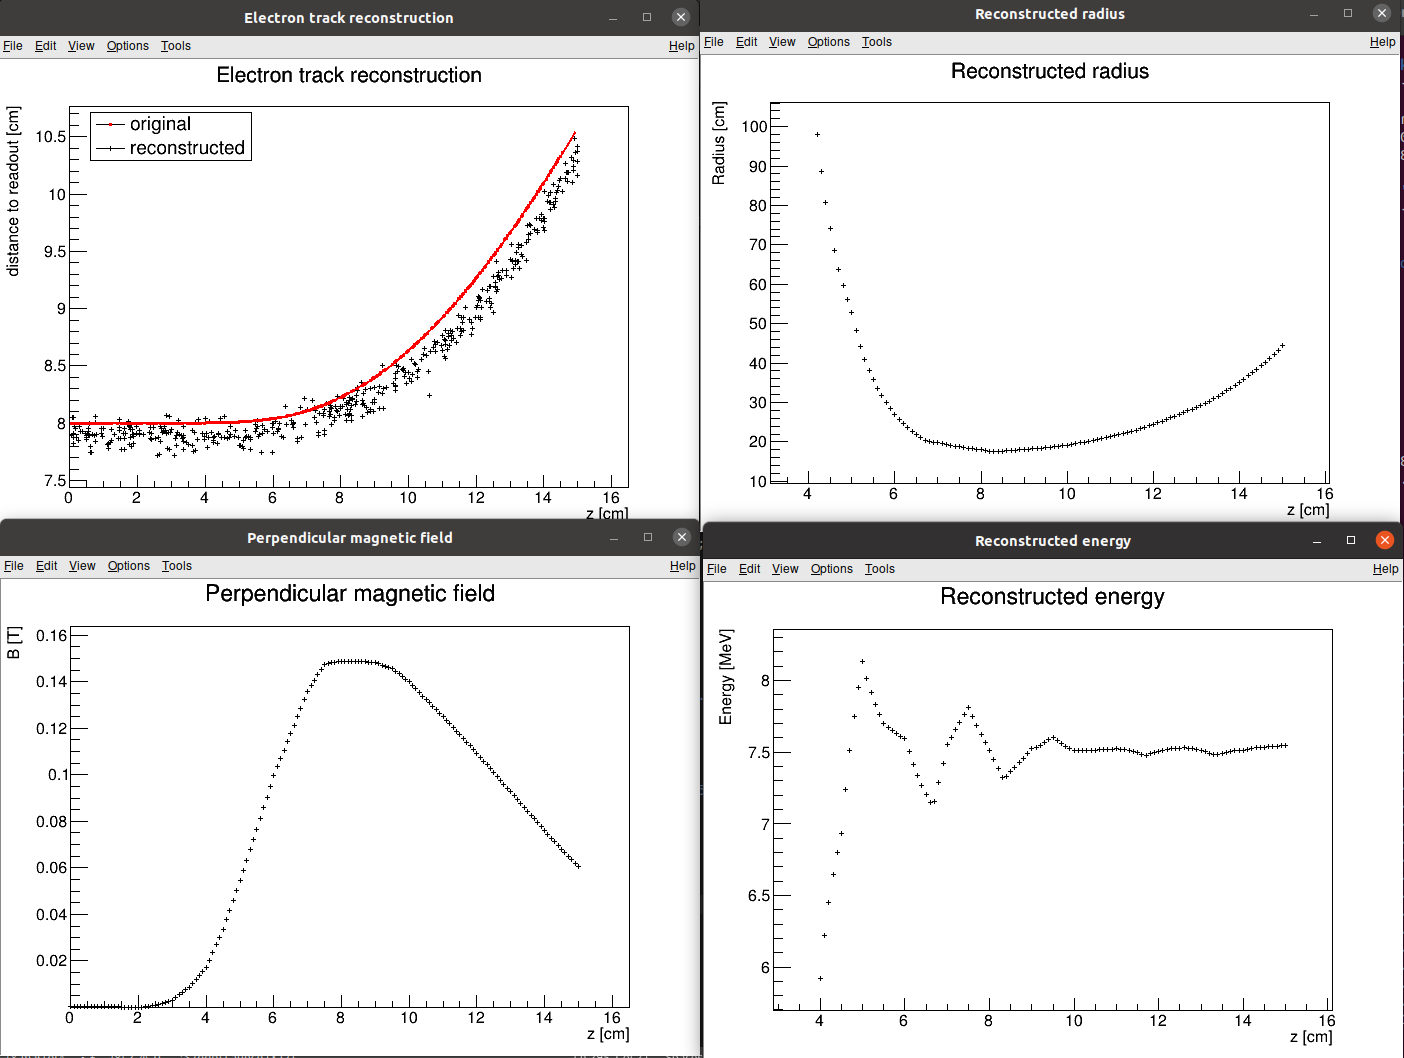
\includegraphics[width=0.8\textwidth]{9010_splines.png}
			\caption{First attempt at a~track reconstruction using only the~drift velocity. Spline energy reconstruction attempt. \textcolor{red}{Swap for better image(s) -- subfigure environment., correct coordinates.}}
			\label{fig:9010splines}
		\end{figure}
	
	\section{Circle and Lines Fit}
	\label{sec:clines}
		\textcolor{red}{Energy reconstruction with circle and lines fit. Trilinear interpolation of the magnetic field. Tested on Runge-Kutta sample, future testing with microscopic simulations and map simulation. Preliminary 2D version and complete 3D version. Geometry of the fit with its derivation.}
		
		\begin{figure}
			\centering
			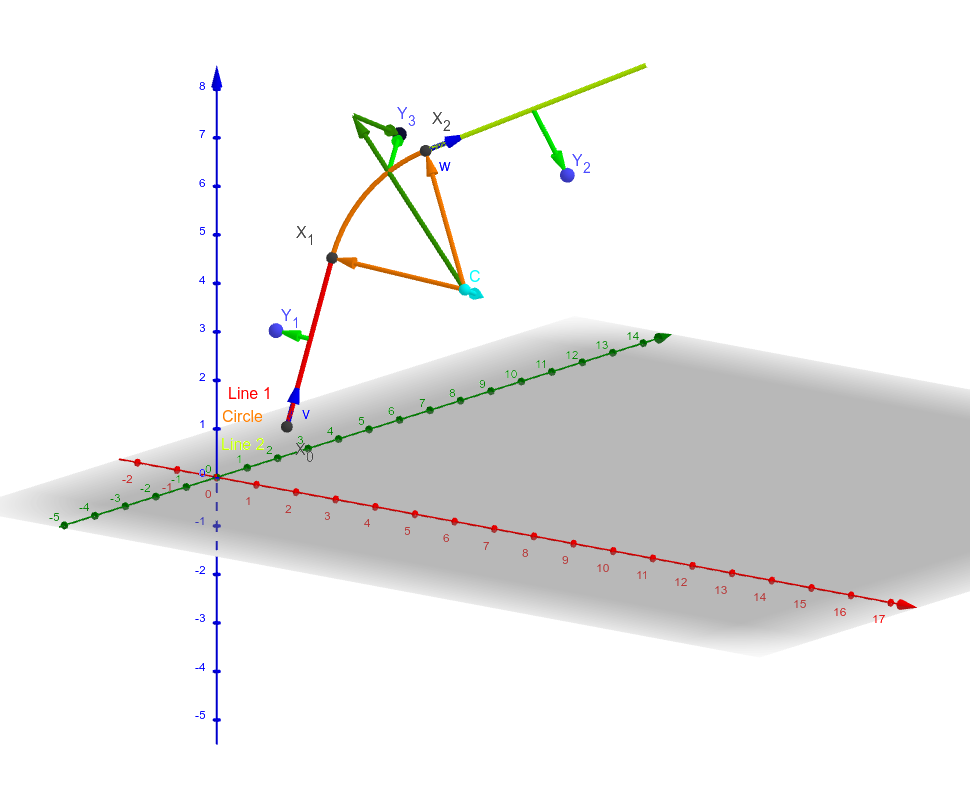
\includegraphics[width=0.8\textwidth]{circlefit.png}
			\caption{Circle and Lines Fit 3D geometry. \textcolor{red}{Swap for better image.}}
			\label{fig:circlefit}
		\end{figure}
		
		\begin{figure}
			\centering
			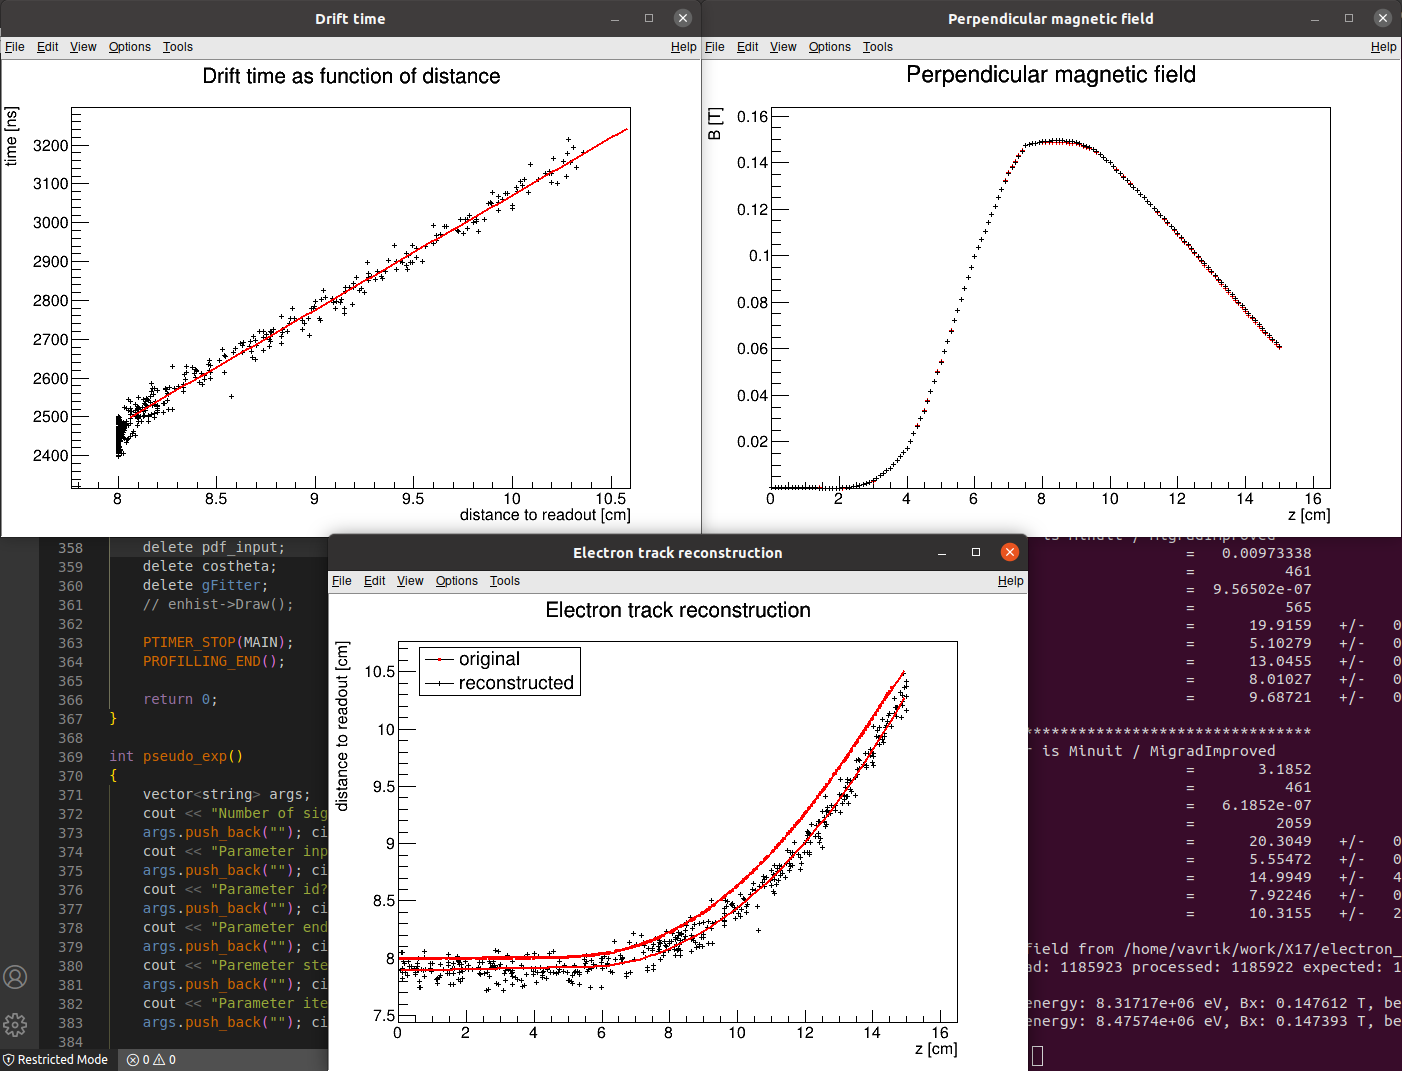
\includegraphics[width=0.8\textwidth]{9010_circle2D.png}
			\caption{First attempt at a~track reconstruction using only the~drift velocity. Circle and Lines Fit in 2D. \textcolor{red}{Swap for better image, correct coordinates.}}
			\label{fig:9010circle2D}
		\end{figure}
	
	\section{Runge-Kutta Fit}
		\textcolor{red}{Single parameter fit with 4th order Runge-Kutta simulated track. Future testing with microscopic simulations and map simulation. Derivation of the geometry (least squares).}